%% ============================================================
%% 分片 28：原文第 10 节「The Bogomolny Equations And The Space Of Hecke Modifications」（原文 glshort.tex 起于第 8120 行）
%% 由 tools/harvmac2tex.py 从 arXiv 源码（hep-th/0604151v3）自动生成。
%% 只译英文散文；公式、编号、\label、\cite 一律不改。
%% ============================================================

\subsection{Kähler 结构与 moment map}

\label{sec:kahstr}

我们的下一个目标是证明 ${\EUZ}({}^L\negthinspace
w_1,\dots,{}^L\negthinspace w_n)$ 是一个 Kähler 流形，并且使其复
结构与第~\ref{sec:thooftheckeop}~节所述、相应的 Hecke 修正模空间
一致。这一分析会使许多事情变得更清楚。它将为我们定义 ${\EUZ}$ 时
所采用的边界条件的选择提供新的动机；它将为理解 't Hooft 算子与
Hecke 算子之间的关系提供更精确的框架；它还将使 Hecke 修正空间的
奇点性质变得更加透明。

\begin{figure}[htbp]
\centering
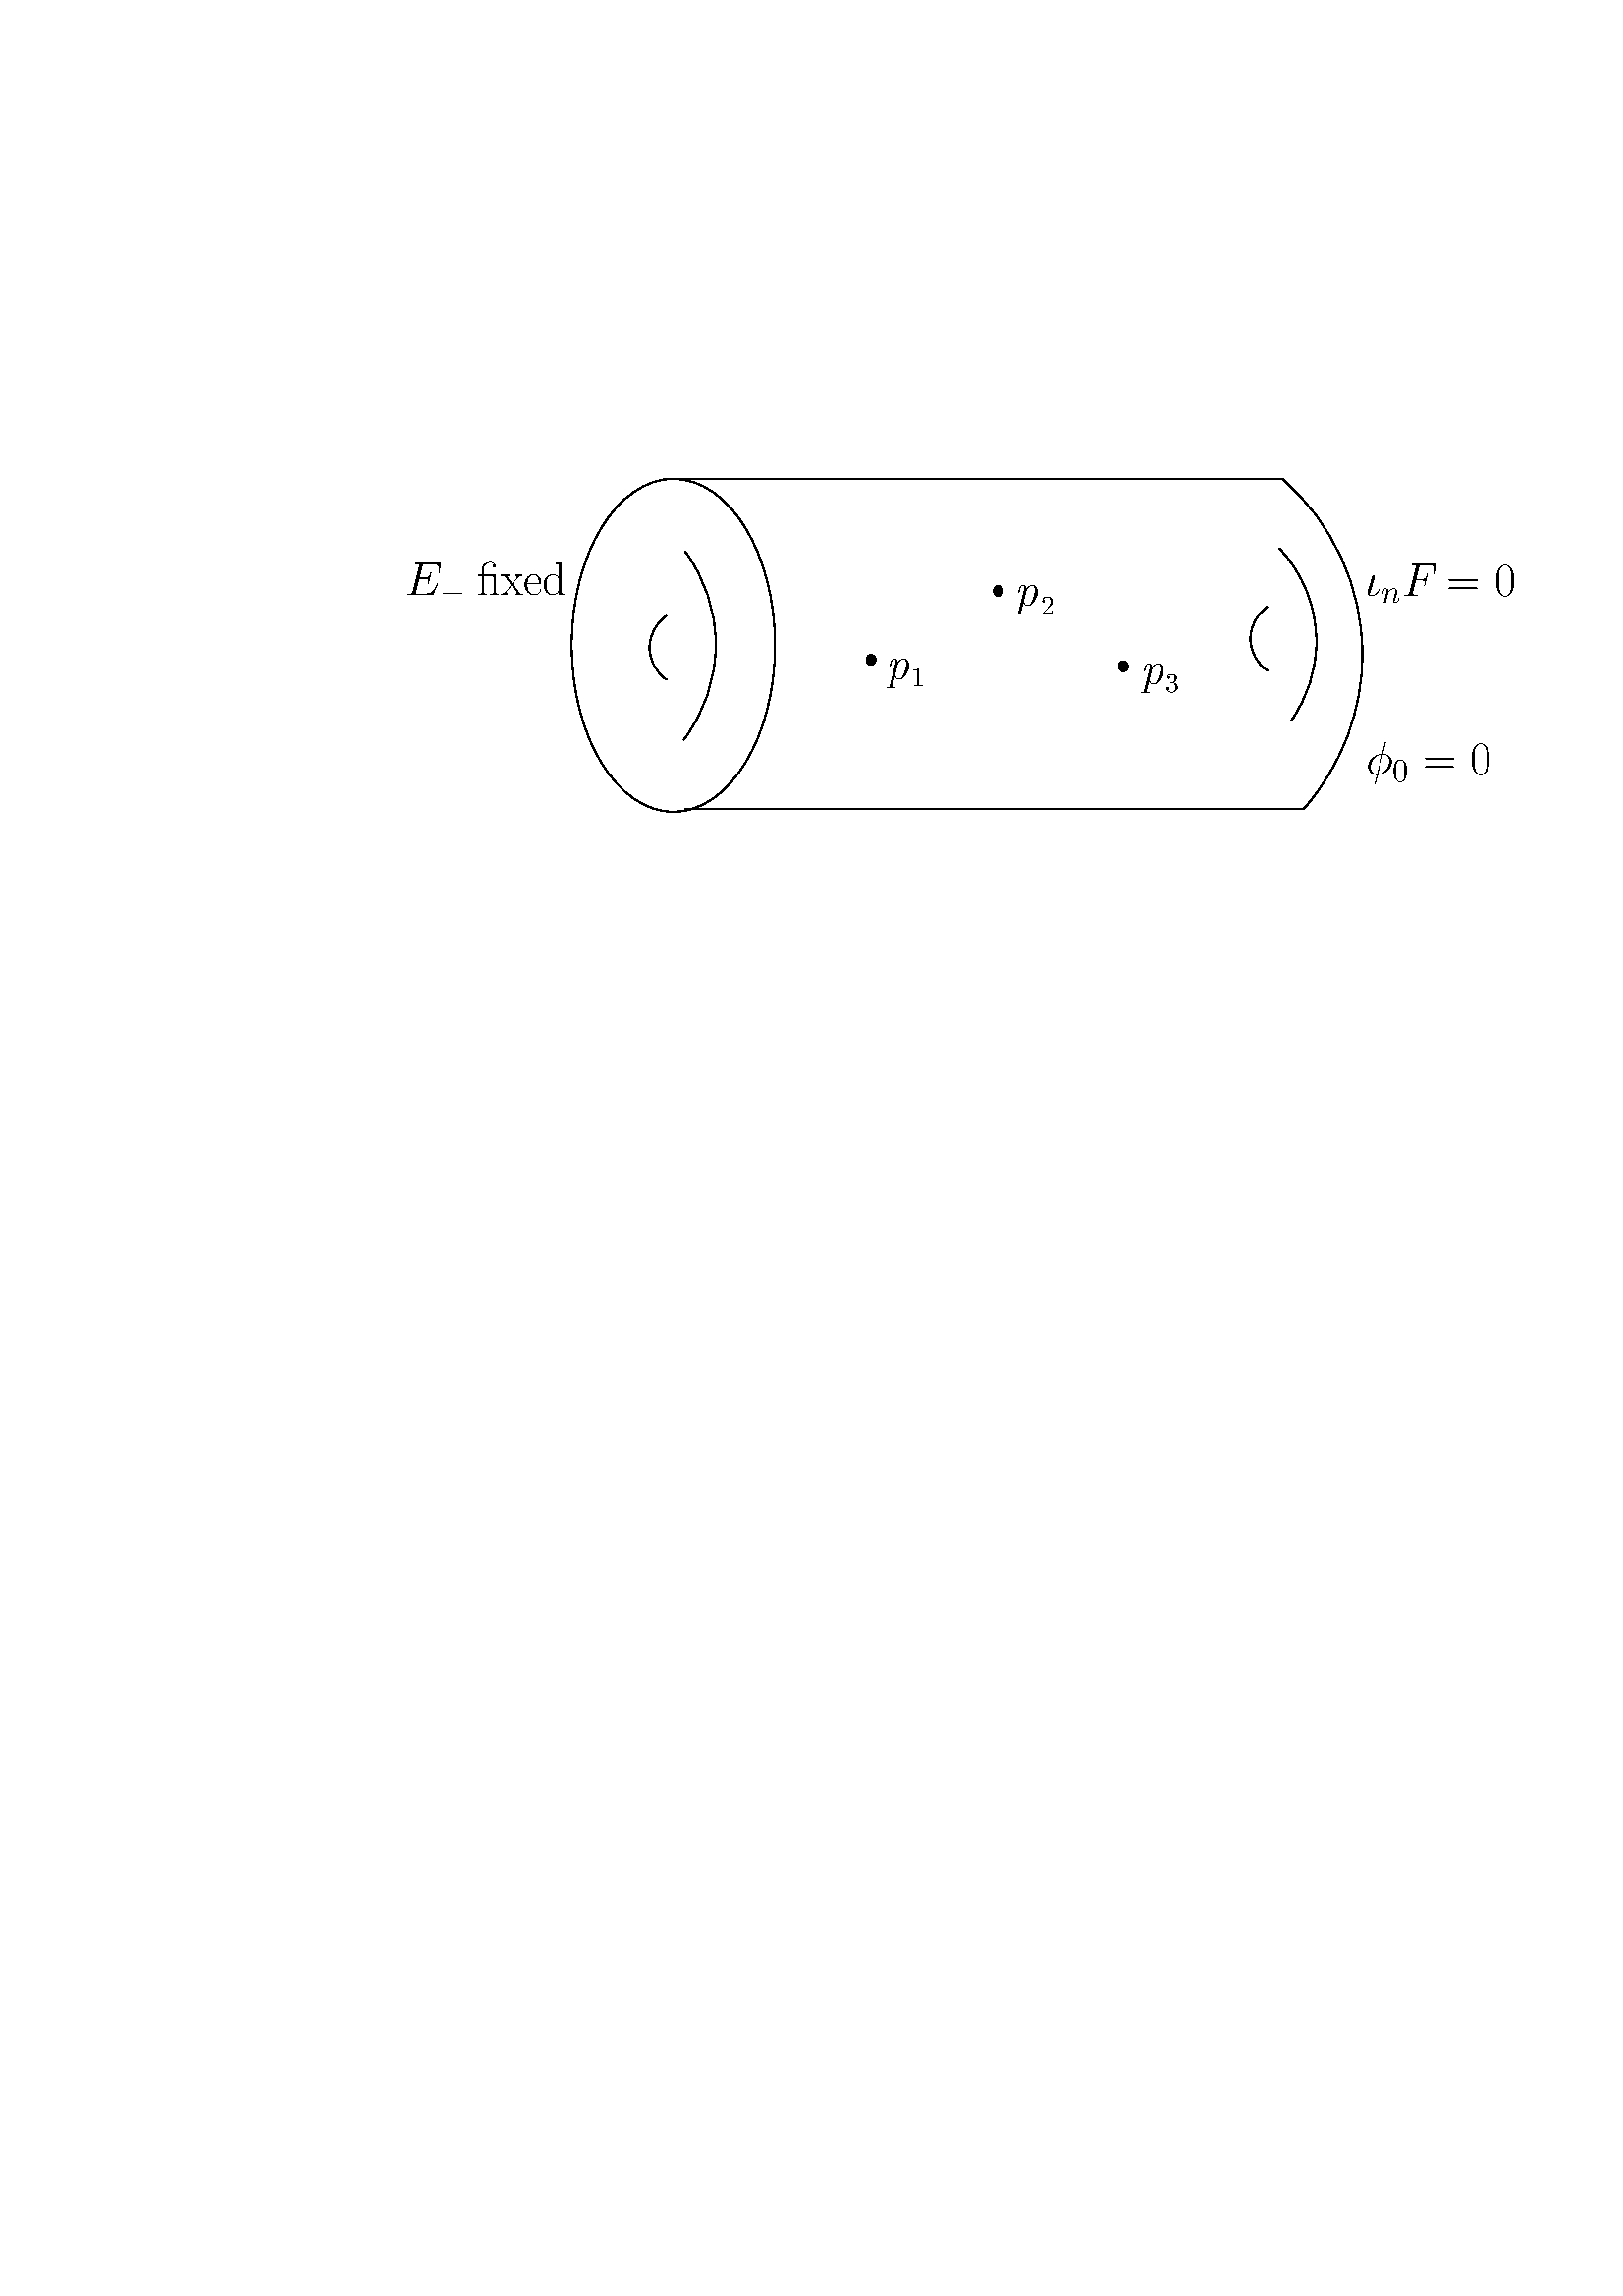
\includegraphics[width=0.75\linewidth]{figures/gla7-5.png}
\caption{在三流形 $W=I\times C$ 上比较 't Hooft 算子与 Hecke 算子。左端给定了联络 $A$ 与丛 $E_-$，并要求规范变换为平凡；右端置 $\phi_0=0$ 并对 $E_+$ 求解。（原文 Fig.~16）}
\label{fig:xutampo}
\end{figure}

正如第~\ref{sec:thooftheckeop}~节引言中那样，我们取三流形
$W=I\times C$ 的度量为 $ds^2=h|dz|^2+dy^2$ 的形式，其中
$z=x^2+ix^3$ 是 $C$ 上的局部复坐标，$y$ 参数化 $I$。我们考虑
Bogomolny 方程 $F=\star D\phi_0$，其中 $F$ 是 $G$-丛 $E$ 上联络
$A$ 的曲率。在 $W$ 的左端，我们指定一个平坦 $G$-丛 $E_-$，并且
只对在边界上等于 1 的规范变换取商；在右端，我们要求
$\phi_0=0$，并对所有规范变换取商。

我们把联络展开为
$A=A_z dz+A_{\bar z}d\bar z+A_ydy=A_2dx^2+A_3
dx^3+A_ydy$。改写 \eqref{eq:noffo}\ 与 \eqref{eq:jungol} 之后，
Bogomolny 方程在这些坐标下可以写成一个复方程 % 式 (10.14)
\setcounter{equation}{13}
\begin{equation}\label{eq:mirot}
\left[D_y-i\phi_0, D_{\bar z}\right]=0
\end{equation}
 与一个实方程 % 式 (10.15)
\setcounter{equation}{14}
\begin{equation}\label{eq:irot}
F_{23}=hD_y\phi_0.
\end{equation}

在域 $(A,\phi_0)$ 构成的空间 ${\EUC}$ 上，我们引入复结构
${\cal I}$，其复坐标为 $A_{\bar z}$ 与 $B=A_y-i\phi_0$。这样
选择的理由是：\eqref{eq:mirot}\ 中的复方程在这个复结构下是全纯
的。此外，我们给 ${\EUC}$ 赋予辛结构 % 式 (10.16)
\setcounter{equation}{15}
\begin{equation}\label{eq:uryt}
\omega=\int_{W}\Tr\Bigl(\delta A_2\wedge
\delta A_3-h\,\delta A_1\wedge \delta\phi_0\Bigr) dx^2\,dx^3\,dy.
\end{equation}

复结构 ${\cal I}$ 与辛结构 $\omega$ 合起来构成一个 Kähler 结构，
其 Kähler 度量为
% 式 (10.17)
\setcounter{equation}{16}
\begin{equation}\label{eq:ryt}
-\int_W\Tr\Bigl( \delta A_2\otimes \delta A_2+\delta
A_3\otimes \delta A_3+h\,\delta A_y\otimes \delta A_y+h\,\delta
\phi_0\otimes \delta \phi_0\Bigr)dx^2\,dx^3\,dy.
\end{equation}

现在我们来求规范群作用的 moment map $\mu$。照例，辛向量场 $v$
的 moment map $\mu(v)$ 由
% 式 (10.18)
\setcounter{equation}{17}
\begin{equation}\label{eq:charby}
d\mu(v)=\iota_v\omega,
\end{equation}
 刻画，其中 $\iota_v$ 是「与 $v$ 缩并」的运算。对于由无穷小
规范变换 $\delta A=-D\epsilon$ 与
$\delta\phi_0 =[\epsilon,\phi_0]$（其中
$\epsilon\in \Omega^0(C,{\rm ad}(E))$）所刻画的向量场，求得
moment map 为 % 式 (10.19)
\setcounter{equation}{18}
\begin{equation}\label{eq:prigo}
\mu(\epsilon)=\int_W\Tr\left(\epsilon(
\,F_{23}-hD_y\phi_0)\right)dx^2\,dx^3\,dy+ \int_{\partial
W}\,\Tr\,(\epsilon\phi_0) \,h\,dx^2\,dx^3.
\end{equation}
 计算与推导式 \eqref{eq:joget} 时类似，只是分部积分时会多出一个
边界项。

当在点 $p_i\in W$ 处有 't Hooft 算子时，我们略微修改这些定义。
要求 $A$ 与 $\phi_0$ 在 $p_i$ 附近具有指定的奇异性。并且约束
$\epsilon$ 在 $p_i$ 附近生成保持所选奇异性不变的规范变换。在这种
情形下，我们的 moment map 公式仍然成立。

我们希望把实 Bogomolny 方程 \eqref{eq:irot}\ 解释为 moment map
取零。事实上，$\mu(\epsilon)$ 为零确实给出 \eqref{eq:irot}，
并附带另一个条件：$\Tr\,\epsilon\phi_0$ 必须在边界上为零。在
$W$ 的任一边界分支 $C_\pm$ 上，有两种简单办法保证
$\Tr\,\epsilon\phi_0=0$。可以令边界上 $\epsilon=0$，也就是只允许
在该边界分支上为平凡的规范变换；也可以令 $\phi_0=0$。为定义模
空间 ${\EUZ}$，我们（\xutampo）在 $C_-$ 上用了其中一种边界条件，
在 $C_+$ 上用了另一种。这样我们就为边界条件找到了新的理由：它们
是最简单的、能把 Bogomolny 方程解释为一个全纯方程加 moment map
取零的条件。

现在我们可以援引辛商与复商之间通常的对应。设 ${\EUC}_0$ 是
${\EUC}$ 中由全纯 Bogomolny 方程 \eqref{eq:mirot}\ 的零点所刻画
的子空间。模空间 ${\EUZ}$ 定义为令 $\mu$ 为零并对 $G$-值规范
变换群 ${\cal G}$ 取商。我们可以把它与
${\EUZ}'={\EUC}_0/{\cal G}_{\Bbb{C}}$ 相比较，后者是 ${\EUC}_0$
对 $G_{\Bbb{C}}$-值规范变换构成的复化群
${\cal G}_{\Bbb{C}}$ 的商。

当然，由于边界条件，${\cal G}$ 是在 $W$ 左端为平凡的规范变换群；
同样，${\cal G}_{\Bbb{C}}$ 是在该端为平凡的
$G_{\Bbb{C}}$-值规范变换群。

通常，在把辛商与相应的复商作比较时，必须担心可能出现的不稳定与
半稳定轨道。然而在本情形中，由于规范变换被限制为在 $W$ 的一端
平凡，这类问题不会出现。${\cal G}_{\Bbb{C}}$ 自由作用且轨道是
闭的，所以所有轨道都是稳定的，从而 ${\EUZ}={\EUZ}'$。

分析 ${\EUZ}'$ 是直截了当的。事实上，我们在
第~\ref{sec:theck}~节中已经基本上做了这件事。对任何远离某个
't Hooft 算子所在位置的 $y\in I$，置
$E_y=E|_{ \{y\}\times C}$。复 Bogomolny 方程表明，只要不越过
't Hooft 算子的位置，$E_y$ 的全纯型就与 $y$ 无关。而且，在没有
't Hooft 算子的区间内，这个全纯型是唯一的
${\cal G}_{\Bbb{C}}$-不变量。在跨过 't Hooft 算子时，$E_y$ 经历
Hecke 修正。所以 ${\EUZ}'$ 就是 $E_-$ 在指定奇异性作用下的
Hecke 修正空间。

这样一来，复商与辛商的比较为理解 't Hooft 算子与 Hecke 算子之间
的关系提供了一个精确的框架——我们在第~\ref{sec:theck}~节中只是
不那么正式地作过这种比较。此外，它还将使我们更好地理解
第~\ref{sec:spaceheck}~节中描述过的 Hecke 修正空间的某些性质。

\par\medskip{\it 改变复结构与辛结构}

我们把 $W=I\times C$ 中插入 't Hooft 算子的点 $p_i$ 记作
$y_i\times z_i$，其中 $y_i\in I$、$z_i\in C$。我们想了解模空间
${\EUZ}$ 对点 $p_i$ 的依赖关系。

引入修正后的联络 $A'=A-i\phi_0 dy$ 会很方便。其想法是：若把
$A'=dz\,A'_z+d\bar z \,A'_{\bar z} +dy\, A'_y$ 展开，
则 $A'{}_y$ 与 $A'{}_{\bar z}$ 在复结构 ${\cal I}$ 下是全纯的，
尽管 $A'_z$ 不是。由于 $A$ 是实的，即取值于 $G$ 的实李代数，
$A'_z$（它等于 $A_z$）是 $A'_{\bar z}$ 的复共轭；当然，$A'_y$
不受任何实性条件约束。要描述群在 $(A,\phi_0)$ 对构成的空间
${\EUC}$（它与修正联络 $A'$ 的空间相同）上的全纯作用，只需描述
$A'_{\bar z}$ 与 $A'_y$ 如何变换。$A'_z$ 的变换则由它是
$A'_{\bar z}$ 的复共轭这一事实确定。

把 $W=I\times C$ 看作 $C$ 上的纤维丛，设 $D_I$ 是 $W$ 的保持该
纤维化的微分同胚群。这样的微分同胚在保持 $z$ 不动的同时把 $y$
映到 $\tilde y(y;z,\bar z)$，其中 $\tilde y$ 在 $W$ 的边界上与
$y$ 一致，且 $\partial \tilde y/\partial y>0$。我们如下定义
$D_I$ 在 ${\EUC}$ 上的作用：直接说 $A'_{\bar z}$ 与 $A'_y$ 按
「拉回」的自然方式变换。

注意，我们不能用拉回来变换 $A'$；对 $\beta\in D_I$，运算
$A'\to \beta^*(A')$ 不会保持 $A'_z$ 与 $A'_{\bar z}$ 互为复共轭
这一事实。我们改而定义
$\beta(A')=\beta^*(A')+dz\,\varepsilon$，其中 $\varepsilon$ 由
保持 $A'_z$ 与 $A'_{\bar z}$ 互为复共轭这一条件确定。

$D_I$ 在 $(A,\phi_0)$ 对构成的空间 ${\EUC}$ 上的这个作用保持复
结构 ${\cal I}$。它也保持复 Bogomolny 方程，因而保持该方程解的
空间 ${\EUC}_0$。这些陈述依赖于 $D_I$ 中微分同胚保持 $z$ 不动
这一事实。因此它们保持由 $\partial/\partial y$ 与
$\partial/\partial \bar z$ 生成的叶状结构，而「沿该叶状结构的叶
平坦」这一断言——正是复 Bogomolny 方程的内容——是不变的。此外，
$D_I$ 把 ${\EUC}$ 的 $G_{\Bbb{C}}$-值规范变换群
${\cal G}_{\Bbb{C}}$ 映到自身。所以由
${\EUZ}={\EUC}_0/{\cal G}_{\Bbb{C}}$ 定义为复流形的 ${\EUZ}$
在 $D_I$ 下不变。

然而，${\EUC}$ 上的辛形式 $\omega$ 肯定不是 $D_I$-不变的，
相应地，${\cal G}$ 作用的 moment map 以及实 Bogomolny 方程也
不再具有不变性。所以，把 ${\EUZ}$ 理解为用辛结构 $\omega$ 对
${\EUC}_0$ 作 ${\cal G}$ 作用的辛商时，它不是 $D_I$-不变的。

结论是：${\EUZ}$ 的复结构是 $D_I$-不变的，但其辛结构不是。

现在考虑位于点 $p_i=y_i\times z_i$ 的 't Hooft 算子。群 $D_I$
可以沿 $y$ 方向上下滑动这些 $p_i$，方式任意，只有一个限制：若
两个 $p_i$ 处于同一个 $z$ 值，则它们在 $y$ 方向上的顺序是
$D_I$-不变的。结论是：沿 $y$ 方向滑动这些 $p_i$（同时不让 $z$
相同的两个点互相越过）会改变 ${\EUZ}$ 的辛结构，但不改变其复
结构。

这件事有一个反向的版本。${\EUC}$ 辛结构的定义只用到 $C$ 的面积
形式，而不用其复结构。因此 moment map $\mu$ 也同样如此。于是，
只给定 $C$ 的面积形式，我们就可以定义辛商
${\EUC}/\negthinspace/{\cal G}=\mu^{-1}(0)/{\cal G}$。这是一个
无穷维辛流形，其辛结构只依赖于 $C$ 的面积形式。一般而言，在辛
流形中，由一族变动的方程所定义的一族辛子流形具有固定的辛结构。
在我们的应用中，变动的这族方程是复 Bogomolny 方程，它们依赖于
$C$ 的复结构。所以当复结构与各点的位置变动时，${\EUZ}$ 的复
结构可以改变，但辛结构不变。

若 't Hooft 算子插入在点 $p_i=y_i\times z_i\in I\times C$，则在
固定 $y_i$ 的前提下改变 $z_i$（并且不改变任一对 $i,j$ 是否有
$z_i=z_j$），等价于改变 $C$ 的复结构的一个特例。所以这样改变
$z_i$ 会改变 ${\EUZ}$ 的复结构，但不改变其辛结构。

\par\medskip{\it 与全纯结果的比较}

我们可以利用这些观察，对第~\ref{sec:spaceheck}~节中描述过的一些
事实获得新的视角。

\begin{figure}[htbp]
\centering
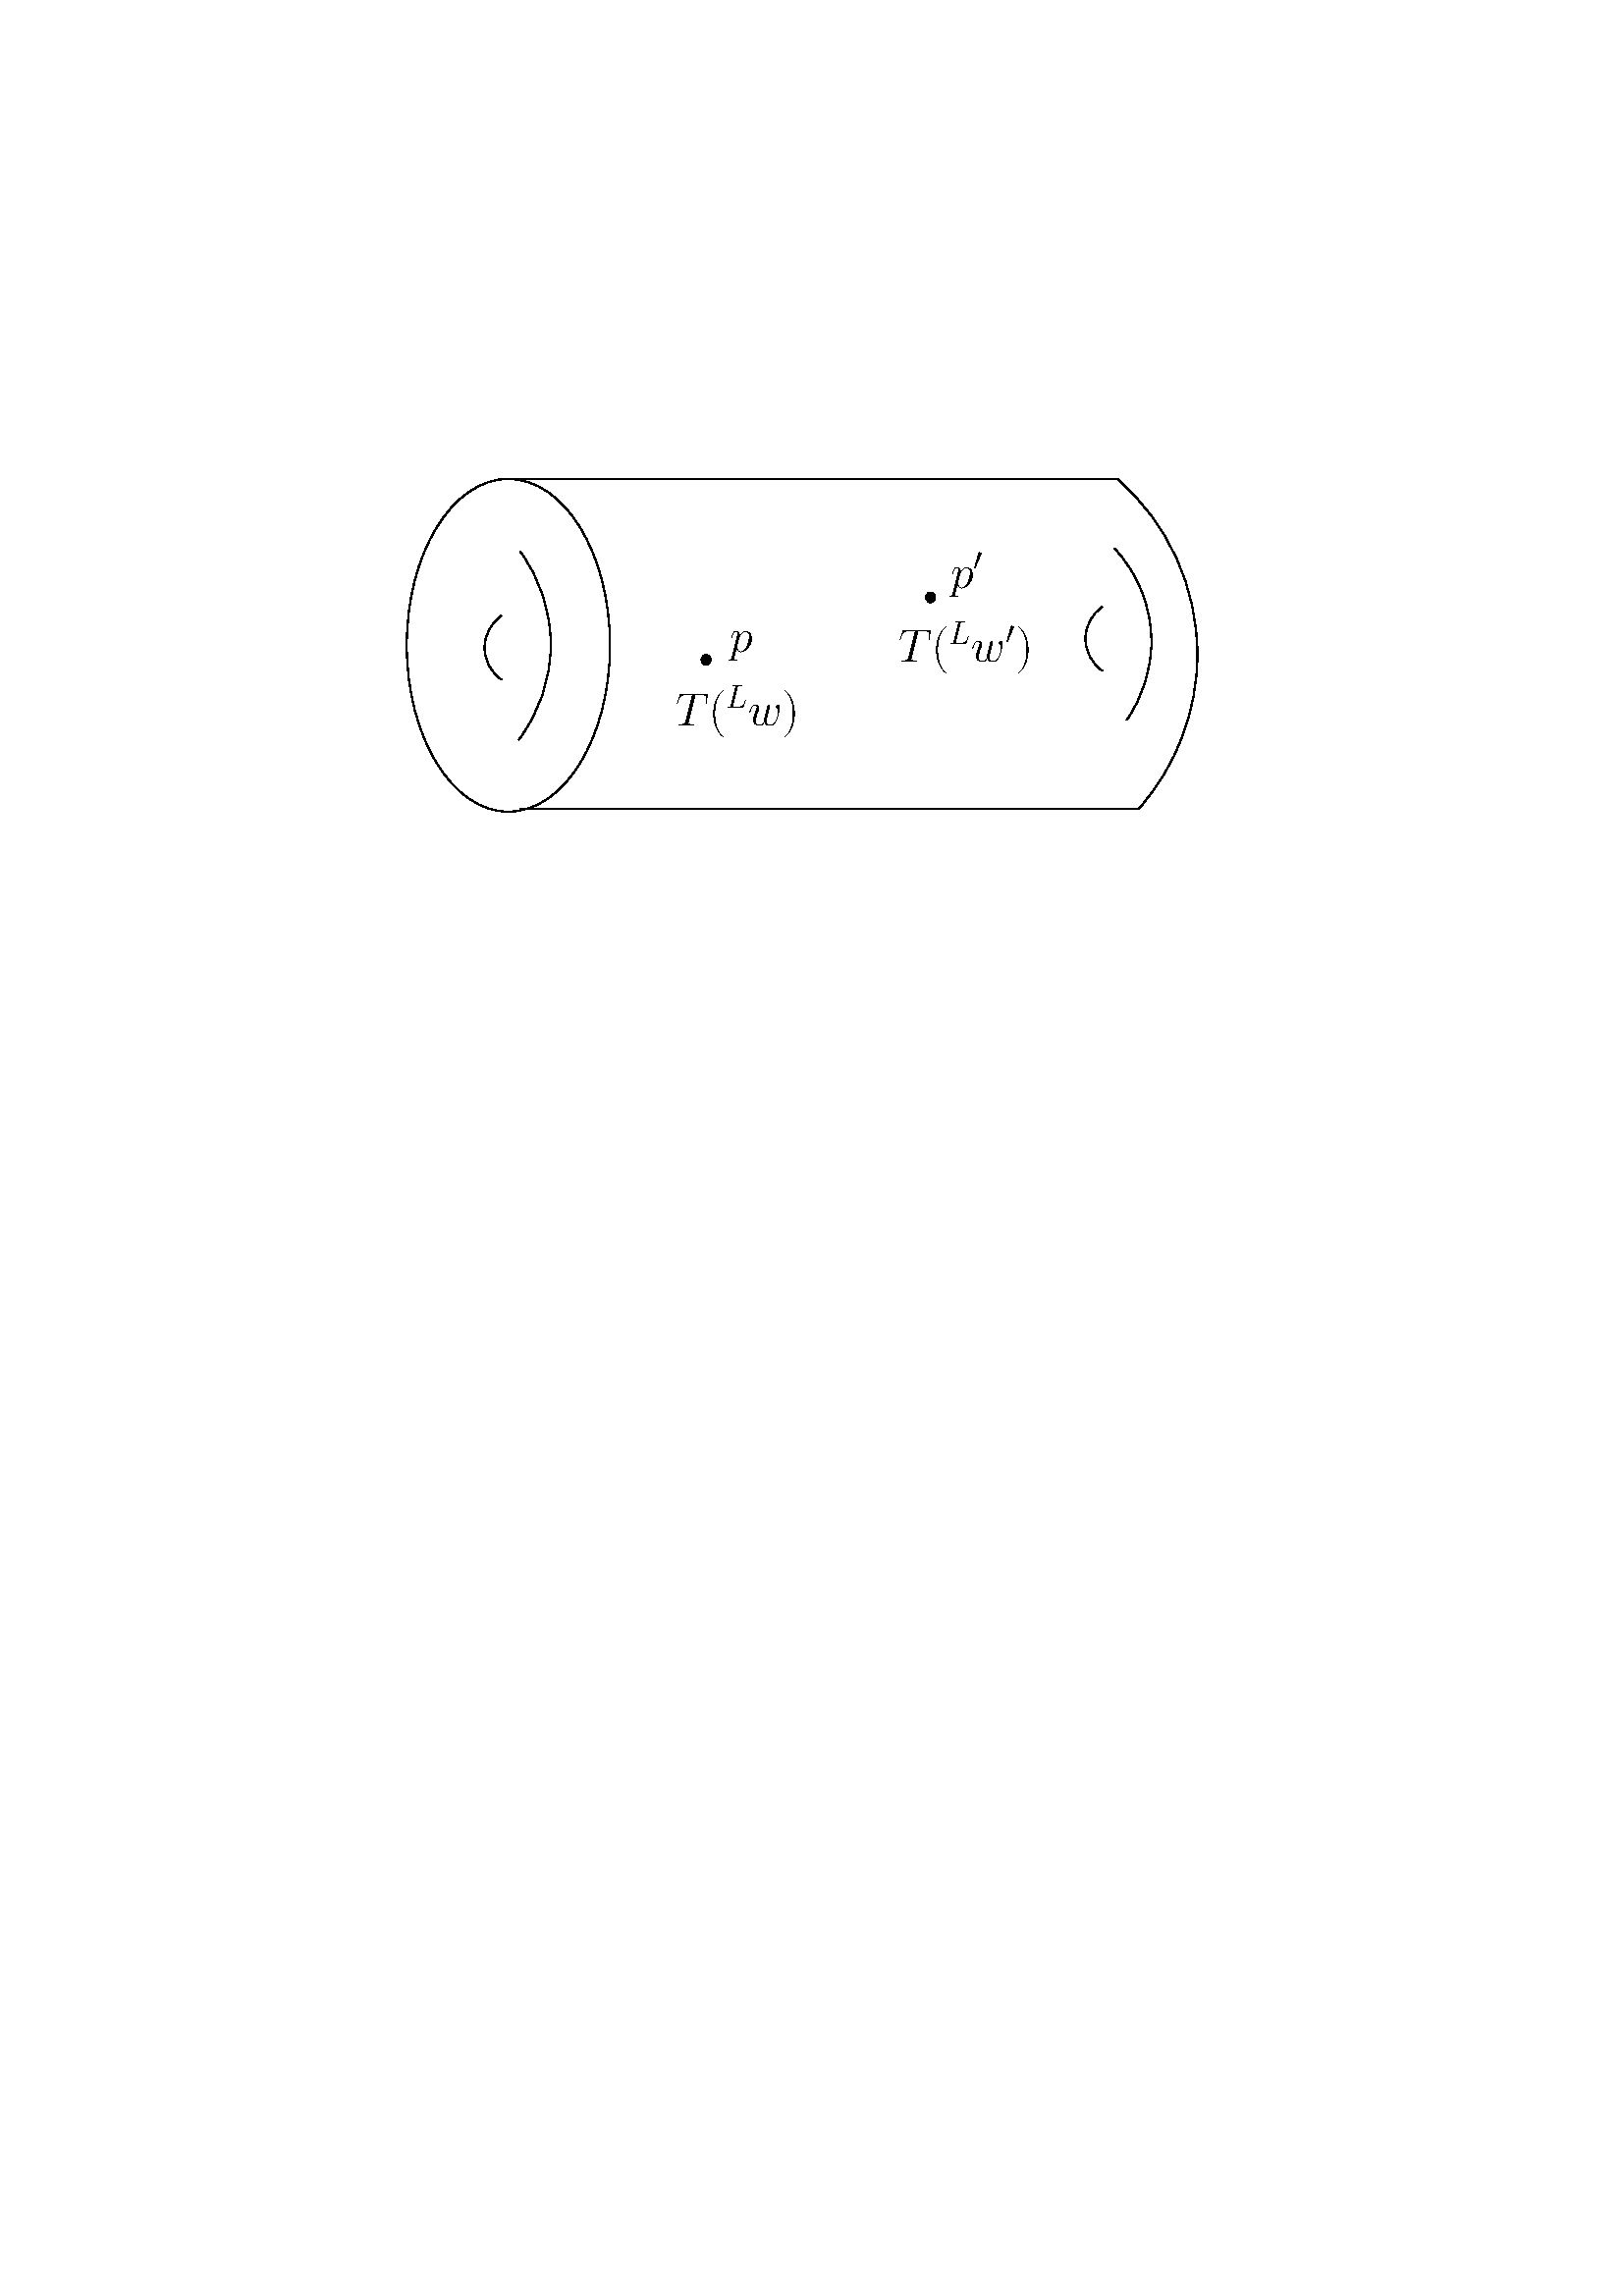
\includegraphics[width=0.75\linewidth]{figures/gla7-6.png}
\caption{在点 $p,p'\in W$ 处插入两个权为 $^L\negthinspace w$ 与 $^L\negthinspace w'$ 的 't Hooft 算子。（原文 Fig.~17）}
\label{fig:xtampo}
\end{figure}

考虑 $W=I\times C$，在其中插入两个指定权的 't Hooft 算子
$T(^L\negthinspace w,p)$ 与 $T(^L\negthinspace w',p')$，插入点为
$p=y\times z$ 与 $p'=y'\times z'$（\xtampo）。我们把相应的紧化
模空间（在 $W$ 左端取某个指定的丛 $E_-$）记作
$\bar{\EUZ}(^L\negthinspace w,p;{}^L\negthinspace w',p')$，或更
简短地记作 $\bar{\EUZ}(p;p')$；同样，把只有一个奇点的类似
Bogomolny 模空间记作 $\bar{\EUZ}(^L\negthinspace w,p)$。

我们可以通过沿 $I$ 方向移动各点（保持到 $C$ 的投影不变）来改变
$\bar\EUZ(p;p')$ 的辛结构；也可以通过沿 $C$ 方向移动各点（保持
到 $I$ 的投影不变）来改变其复结构。

一般来说，$\bar\EUZ(p;p')$ 是奇异的。甚至与单个 't Hooft 算子
（例如 $T(^L\negthinspace w_1)$ 或 $T(^L\negthinspace w_2)$）
相伴的 Hecke 修正模空间也一般是奇异的，正如我们在
第~\ref{sec:spaceheck}~节所讨论的。例外情形对应于
$^L\negthinspace G$ 的极小表示（minuscule representation）。

所以即使 $p\not= p'$，$\bar{\EUZ}(p;p')$ 通常也是奇异的。但当
$p'\to p$ 时它变得更奇异（若原先光滑则产生奇点）。我们把
$p'\to p$ 时的奇异极限记作 $\bar\EUZ{}^*$。我们可以通过沿 $I$
方向移动各点来部分消解 $\bar\EUZ{}^*$ 的奇点，也可以沿 $C$ 方向
移动各点来部分形变这些奇点（\xdtampo）。这种奇点的部分形变与
部分消解在拓扑上是等价的，因为我们可以同时在 $I$ 与 $C$ 两个
方向上移动 $p$ 与 $p'$。

若 $z\not=z'$，则作为复流形 $\bar\EUZ(p;p')$ 是简单乘积
$\bar\EUZ({}^L\negthinspace w,p)\times
\bar\EUZ({}^L\negthinspace w',p')$，它参数化 $C$ 中两个点 $z$ 与
$z'$ 处彼此独立的 Hecke 变换。若 $z=z'$ 且 $y<y'$，则它是
$\bar\EUZ({}^L\negthinspace w,p)$ 上的纤维丛，纤维为
$\bar\EUZ({}^L\negthinspace w',p')$，描述 $E_-$ 在点
$z\in C$ 处依次进行权为 $^L\negthinspace w$ 与
$^L\negthinspace w'$ 的 Hecke 修正。若 $z=z'$ 且 $y'<y$，则
$\bar\EUZ(p;p')$ 仍是纤维丛，只是 $^L\negthinspace w$ 与
$^L\negthinspace w'$ 的角色互换。

\begin{figure}[htbp]
\centering
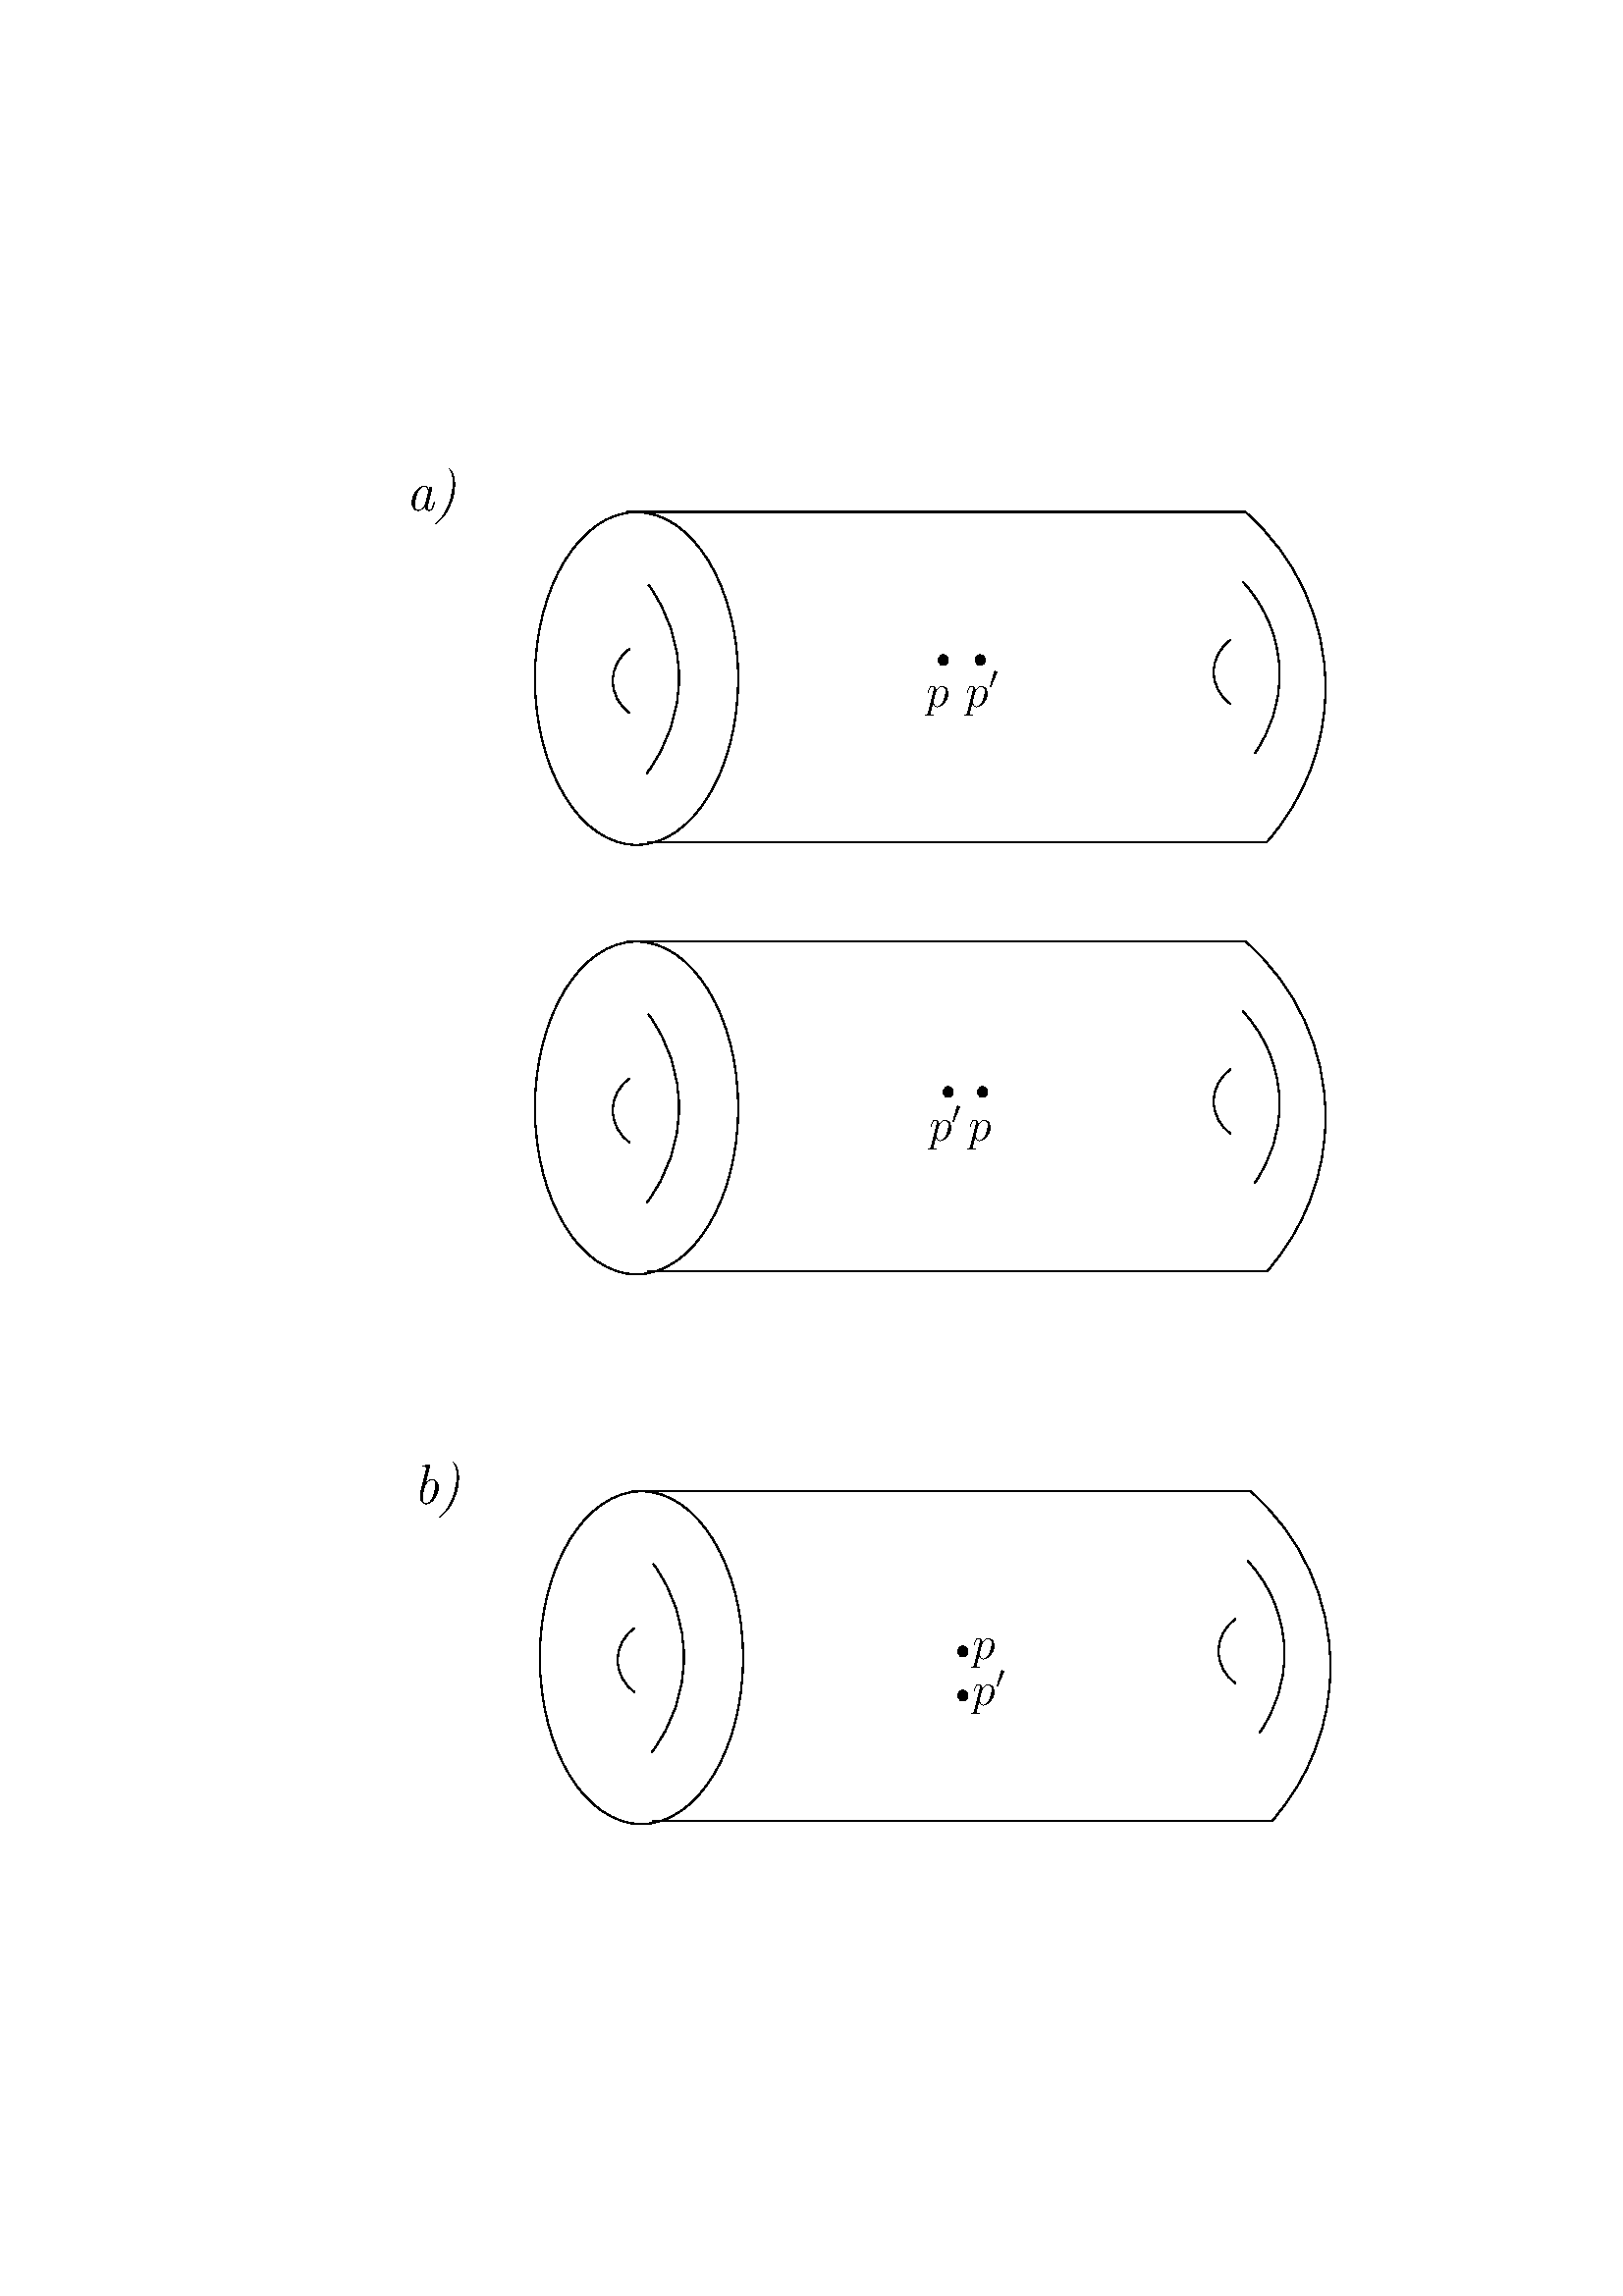
\includegraphics[width=0.75\linewidth]{figures/gla7-7.png}
\caption{（a）奇点的两种部分消解。模空间是一个纤维丛，参数化同一个点 $z\in C$ 处相继的 Hecke 修正。（b）奇点的一种部分形变。模空间是一个乘积，参数化不同点 $z,z'\in C$ 处彼此独立的 Hecke 修正。（原文 Fig.~18）}
\label{fig:xdtampo}
\end{figure}

刚刚描述的、兼有形变与消解的空间 $\bar\EUZ{}^*$ 究竟是什么？
它实际上是 $\bar{\EUZ}(^L\bar w,p')$，即存在单个权为
$^L\bar w={}^L\negthinspace w+{}^L\negthinspace w'$ 的 't Hooft
算子时 Bogomolny 方程解的紧化模空间。

从物理的角度看，这个陈述是算子 $T(^L\negthinspace w,p)$ 与
$T(^L\negthinspace w',p')$ 的算子乘积展开的一部分。我们在
第~\ref{sec:lineop}~节中讨论过这种展开的一些一般性质。那里解释
的简单论证足以说明：乘积 $T(^L\negthinspace w,p)\cdot
T(^L\negthinspace w',p')$ 可以展开为
$\sum_{i\in \EUR}c_i T(^L\negthinspace w_i,p')$，其中
$^L\negthinspace w_i$ 取某个权集 $\EUR$，$c_i$ 为系数。$S$-对偶
预言了该展开的具体形式（它应当与 $^L\negthinspace G$ 的表示环
相吻合），但直接验证这一预言很困难。不过，
第~\ref{sec:lineop}~节中的简单论证确实足以说明：当 $p\to p'$ 时，
展开的形式为
% 式 (10.20)
\setcounter{equation}{19}
\begin{equation}\label{eq:hittor}
T({}^L\negthinspace w,p)\cdot T({}^L\negthinspace
w,p')\to T({}^L\bar w,p')+\sum_{i\in \EUR'} c_i
T({}^L\negthinspace w_i,p'),
\end{equation}
 其中 $^L\bar w={}^L\negthinspace
w+{}^L\negthinspace w'$，而权 $^L\negthinspace
w_i,\,i\in \EUR'$ 是使得 $^L\bar
w-{}^L\negthinspace w_i$ 也为主权的那些主权的权。这意味着
$^L\negthinspace w_i$ 就是我们所说的 $^L\bar w$ 的相伴权重
（associated weight）。

公式 \eqref{eq:xinon} 表明，$\bar\EUZ(^L\bar
w,p')$ 的维数恰好等于
$\bar\EUZ(^L\negthinspace w,p;{}^L\negthinspace w',p')$ 的维数。
这与「前者是后者在 $p\to p'$ 时的极限」这一陈述是一致的。其他
空间 $\bar\EUZ(^L\negthinspace w_i,p')$（$i\in \EUR'$）的维数
严格更小。事实上，在某种意义上，所有空间
$\bar\EUZ(^L\negthinspace w_i,p')$ 都出现在
$\bar\EUZ(^L\negthinspace w,p;{}^L\negthinspace w',p')$ 当
$p\to p'$ 时的极限中。由于这些 $^L\negthinspace w_i$ 是
$^L\bar w_i$ 的相伴权重，按类型 $^L\bar w$ 的 Hecke 修正空间的
自然紧化 $\bar {{\EUY}}(^L\bar w)$ 就包含了所有
$i\in \EUR'$ 的、类型为 $^L\negthinspace w_i$ 的 Hecke 修正空间
$\bar {{\EUY}}(^L\negthinspace w_i)$。用 Bogomolny 模空间的
语言说，这意味着所有空间
$\bar\EUZ(^L\negthinspace w_i,p')$ 都包含在
$\bar\EUZ(^L\bar w,p')$ 的奇异「单极子冒泡」轨迹之中。

这就是为什么确定 't Hooft 算子的算子乘积展开很困难：\eqref{eq:hittor}
中的次领头项全都来自 $\bar\EUZ(^L\bar w,p')$ 的奇点。在
第~\ref{sec:opprod}~节中，我们将解释某些数学结果
\cite{ref97,ref98}，从物理观点看它们等价于确定完整的算子乘积
展开。

不过，我们首先想回顾第~\ref{sec:spaceheck}~节中分析过的一个
例子，它很好地说明了上述论证。取 $G=PSU(2)$、$\LG=SU(2)$、
$^L\negthinspace w={}^L\negthinspace
w'=(1/2,-1/2),$ 以及 $^L\bar w={}^L\negthinspace
w+{}^L\negthinspace w'=(1,-1)$。权 $^L\negthinspace w$ 与
$^L\bar w$ 分别对应于 $\LG=SU(2)$ 的二维表示与伴随表示。正如
我们在第~\ref{sec:spaceheck}~节所知，空间
$\bar {{\EUZ}}(^L\negthinspace w,z)$ 与
$\bar {{\EUZ}}(^L\negthinspace w',z)$ 都是 $\Bbb{CP}^1$ 的拷贝。
空间 $\bar\EUZ{}^*=\bar {{\EUZ}}(^L\bar w,z)$ 是加权射影平面
$\Bbb{WCP}^2(1,1,2)$，具有一个轨形奇点。我们已经发现，这个奇异
空间可以形变为乘积 $\Bbb{CP}^1\times\Bbb{CP}^1$，也可以消解为
一个 Hirzebruch 曲面（它是 $\Bbb{CP}^1$ 上的 $\Bbb{CP}^1$-丛）。
我们还看到，消解与形变是相容的，意思是该 Hirzebruch 曲面可以
形变为 $\Bbb{CP}^1\times\Bbb{CP}^1$。所有这些都与上面的一般论证
相符。（不过在这个特定例子中 $^L\negthinspace w={}^L\negthinspace
w'$，所以两种消解是等价的。）

在这个例子中，把 $^L\bar w$ 写成非零正权之和只有一种方式。一般
地，这样的写法会有若干种，因此沿这些思路对
$\bar {{\EUZ}}(^L\bar w,z)$ 作部分消解与去奇异化就有若干种选择。
对于秩为 $r$ 的单李群 $^L\negthinspace G$，有 $r$ 个基本权
$^L\negthinspace w_\gamma$（$\gamma=1,\dots,r$），使得任何主
权 $^L\bar w$ 都可以用某些非负整数 $t_\gamma$ 唯一地展开为
$^L\bar w=\sum_{\gamma=1}^r t_\gamma {}^L\negthinspace w_\gamma$。
（例如，若 $^L\negthinspace G=SU(r+1)$，则
$^L\negthinspace w_\gamma$ 就是极小表示
$\wedge^\gamma \VV$（$\gamma=1,\dots r$）的最高权。这些表示称为
基本表示。）用 Bogomolny 方程所能做到的、对
$\bar {{\EUY}}(^L\bar w,z)$ 的最大部分消解与去奇异化，就是把它
与一个模空间联系起来：该模空间带有 $t_\gamma$ 个类型为
$^L\negthinspace w_\gamma$ 的 't Hooft 算子插入
（$\gamma=1,\dots,r$）。对 $SU(r+1)$，由于基本表示都是极小的，
这就给出了任意给定权的 Hecke 修正空间的奇点的完全消解或完全
形变。

对其他群，我们能做的最好就是化归为具有基本权的 't Hooft 算子
$T({}^L\negthinspace w_\gamma)$ 的乘积的奇点。这种算子的 Hecke
修正空间带有与单极子冒泡相关的奇点，这些奇点可以局部地用一个
超凯勒流形来模拟，但是对这些奇点没有明显的超凯勒消解。

\begin{yizhu}[易错点]
按：${\cal I}$ 下的复坐标是 $A_{\bar z}$ 与 $B=A_y-i\phi_0$；注意取作
全纯坐标的是 $A_{\bar z}$ 而不是 $A_z$，这与 (10.14) 中 $D_{\bar z}$
所扮演的角色一致。Kähler 度量 (10.17) 带整体负号，是因为 $A$ 与
$\phi_0$ 取值于紧群 $G$ 的李代数，$\Tr$ 在基本表示下负定；只有加上
负号，$\int\Tr(\delta A_i\otimes\delta A_i)$ 才是正定的场空间度量。
另外，(10.16) 中写的是 $\delta A_1$，而 (10.17) 中写的是
$\delta A_y$；由于 $x^1=y$，二者是同一个分量，原文只是记号混用。
\end{yizhu}

\begin{yizhu}[含糊点拨]
按：$\mu(\epsilon)$ 中的边界项
$\int_{\partial W}\Tr(\epsilon\phi_0)h\,dx^2\,dx^3$ 来自分部积分；
正因为有它，$\mu=0$ 才不只给出实 Bogomolny 方程 (10.15)，还要求
边界上 $\Tr\,\epsilon\phi_0=0$。这就是为什么定义 ${\EUZ}$ 时必须
在每个边界分支上二选一：一端令 $\epsilon=0$（只允许平凡的规范
变换），另一端令 $\phi_0=0$。原文只说「有两种简单办法」，其来源
正是这个边界项；而正是这种不对称的选取使得 ${\cal G}_{\Bbb{C}}$
自由作用、轨道闭，从而辛商与复商相等。
\end{yizhu}

\begin{yizhu}[物理图像]
按：$D_I$ 的作用给出「沿 $y$ 移动 = 变辛结构，沿 $z$ 移动 = 变复
结构」的清晰图像。翻成几何语言：把两个 't Hooft 算子在 $C$ 中的
位置分开（$z\ne z'$）得到乘积／形变，把它们重合（$z=z'$）得到
纤维丛／消解。这正对应镜像对称中复结构与辛结构互换的图景：一侧
看到的是复结构的形变，另一侧看到的是辛结构的变分；而
Bogomolny 方程恰好同时提供这两种视角。
\end{yizhu}

\begin{yizhu}[原文疑误]
按：原文「we require $\phi_0=0$ with and divide by all gauge
transformations」中多出一个 with（arXiv v3 源码亦如此），应读作
「require $\phi_0=0$ and divide by all gauge transformations」。
译文按后一读法处理，特此说明。
\end{yizhu}

\begin{yizhu}[原文疑误]
按：本片另有两处原文笔误，均照录：(1) 式 (10.20) 左端第二因子写作
$T({}^L\negthinspace w,p')$，但按上下文（乘积
$T(^Lw,p)\cdot T(^Lw',p')$ 的展开，且 $^L\bar
w={}^Lw+{}^Lw'$）应为 $T({}^L\negthinspace w',p')$；
(2)「Since the $^L\negthinspace w_i$ are associated weights of
$^L\bar w_i$」中的 $^L\bar w_i$ 应为 $^L\bar w$——$\bar w_i$ 在
全文中并无定义，所指的显然是 $^L\bar w$。
\end{yizhu}

\begin{yizhu}[物理图像]
按：'t Hooft 算子的 OPE 有清晰的几何来源：当两个算子互相靠近时，
模空间 $\bar\EUZ(p;p')$ 的极限就是单个算子的模空间
$\bar\EUZ(^L\bar w,p')$，因此领头项是权相加的算符
$T(^L\bar w,p')$；而次领头项来自 $\bar\EUZ(^L\bar w,p')$ 的奇异
轨迹（正是单极子冒泡的所在），故其系数无法由简单论证确定，需要
$S$-对偶／表示环的信息。参见 Frenkel 2009 综述：'t Hooft 函子是
四维 't Hooft 圈算子的二维影子，由「只保持 Higgs 场的那些 Hecke
修正」定义，这与本片边界条件的选取相呼应。
\end{yizhu}

\begin{yizhu}[易错点]
按：极小表示（minuscule）指最高权 $\lambda$ 满足
$\langle\lambda,\alpha^\vee\rangle\le 1$（对一切正根 $\alpha$）
的不可约表示。$SU(r+1)$ 的基本表示 $\wedge^\gamma\VV$ 都是极小的，
故对应的 't Hooft 算子奇点最轻，可由 Bogomolny 方程完全消解。对
一般单李群，基本表示不必极小，于是只能把奇点化归为若干基本权
算子的乘积，而不能再进一步消解——这正是原文最后两段的结论。
\end{yizhu}
